\documentclass[12pt,a4paper]{article}
\usepackage[ngerman]{babel}
\usepackage[T1]{fontenc}
\usepackage[utf8x]{inputenc}
\usepackage{url}
\usepackage{graphicx}
\usepackage{geometry}
\usepackage{amsfonts}
\usepackage{amsmath}
\usepackage{tabularx}
\usepackage{txfonts} %Times New Roman Font
\usepackage{titlesec} %Format der Headings ändern
\usepackage{hyperref}
\usepackage{comment}

\renewcommand{\thesection}{\arabic{section}.} %Nummerierung der Sections anpassen
\renewcommand{\labelenumi}{\alph{enumi})}  %Nummerierung der Listen anpassen
\titleformat{\section}{\large\bfseries}{\thesection}{0.5em}{} %Format der Section Überschrift ändern
\setlength{\parindent}{0pt} %Keine Einrückung bei neuen Paragraphen
\geometry{left=2.0cm,textwidth=17cm,top=2.5cm,textheight=23cm}

% Anpassen %
%%%%%%%%%%%%%%%%%%%%%%%%%%%%%%%%%%%%%
\newcommand{\student}{Max Mustermann\\ 108012345678 } % Namen eintragen
\newcommand{\partner}{Max Mustermann\\ 108012345678} % Matrikelnummer eintragen
\newcommand{\thirdone}{Max Mustermann\\ 108012345678}
\newcommand{\group}{D} % Gruppennummer eintragen
%%%%%%%%%%%%%%%%%%%%%%%%%%%%%%%%%%%%%

\newcommand{\hwheadtwo}{$ $
  \vspace{-2cm}
  
\noindent \student \qquad \qquad  Wireless Physical Layer Security Praktikum \hfill SS 2020 \\
\noindent \partner \\
%\noindent \thirdone \\  % einkommentieren, falls ihr eine 3er Gruppe seid
\noindent Gruppe:~\group\\
$ $

  
\begin{center}    
{\Large \bf Abgabe PHYSEC 2}
\end{center}
}

\begin{document}
\hwheadtwo

\section{FM-Empfänger}

\begin{comment}  
%Fürs erste alles auskommentiert was nicht für Assignment %gebraucht wird, man aber als Vorlage/Orientierungshilfe %benutzen kann


\subsection*{a)}


Zuerst muss inspectrum installiert werden. Als nächstes wird inspectrum gestartet und die mitgegebene file namens SecretSignal.raw geöffnet. %
%
Anschließend wird das Programm mit der rechten Maus-Taste angeklickt: Add derived plot -> Add sample plot.
%
Eine horizontale \glqq Spannweite\grqq \hspace{0.5mm} öffnet sich. Es muss entsprechend mit der Maus angepasst werden. %
% 
Es ist bekannt, dass  Amplitude-Shift Keying, abgekürzt ASK als digitale Modulationsart verwendet wurde. Entsprechend werden Nullen und Einsen zugewiesen, siehe Abbildung~\ref{fig:YourLabe3}.
%
Darüber hinaus ist bekannt, dass die Nachricht mit der Präambel 0x55 anfängt, welche nicht teil der eigentlichen Nachricht ist. %
%
Danach wird in Bytes aufgeteilt und mit ASCII kodiert.


\subsection*{b)}

Die Nachricht besteht aus dem wiederholten String \glqq Money4Physec\grqq. Abfolge: 
0x55, 0x4D, 0x6F, 0x6E, 0x65, 0x79, 0x34, 0x50, 0x68, 0x79, 0x73, 0x65, 0x63, 0x55, 0x4D und so weiter... \\


\begin{figure}[ht!]
\centering
	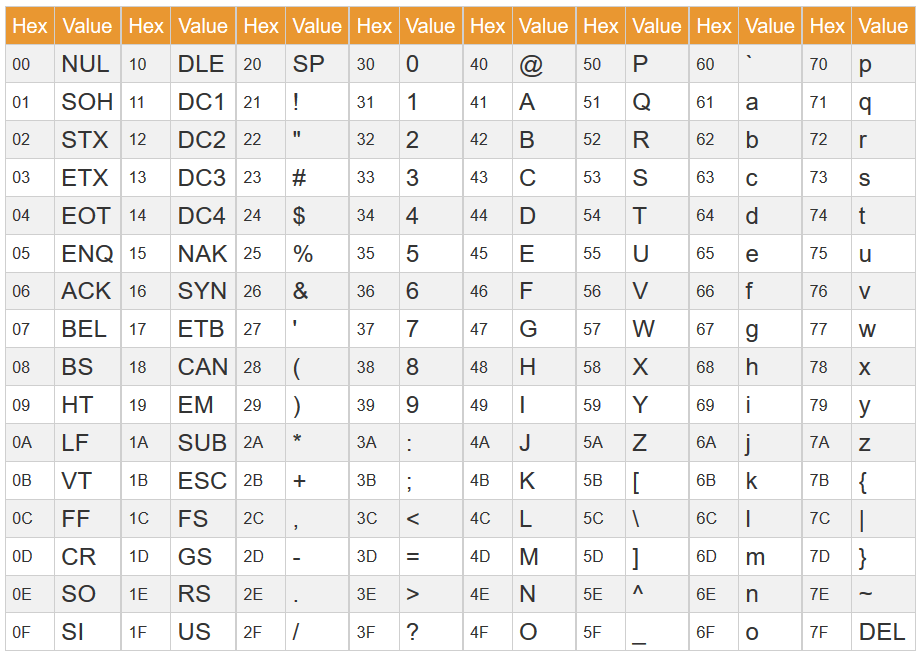
\includegraphics[width=0.77\textwidth ]{images_files/ascii-table.png}
	\caption{\href{https://www.sciencebuddies.org/science-fair-projects/references/ascii-table}{Quelle: Hier klicken}}
	\label{fig:YourLabel}
	
\end{figure}


\newpage


\begin{center}
Diese Tabelle weist jedem Byte die entsprechende ASCII Kodierung zu:

\end{center}

 
\begin{figure}[ht!]
\centering
	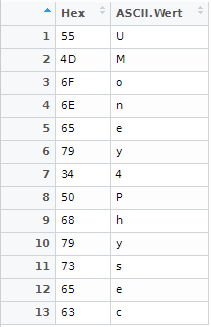
\includegraphics[width=0.7\textwidth ]{images_files/Matrix_Nachricht.png}
	\caption{Tabelle 2}
	\label{fig:YourLabe2}
\end{figure}
 


\newpage
Diese zwei Screenshots zeigen wie der Anfang vom Signal mithilfe von inspectrum analysiert aussieht. Farbige Kodierung sowie Umrandungen wurden hinterher selbst hinzugefügt.\\~\\

\begin{figure}[ht!]
\centering
	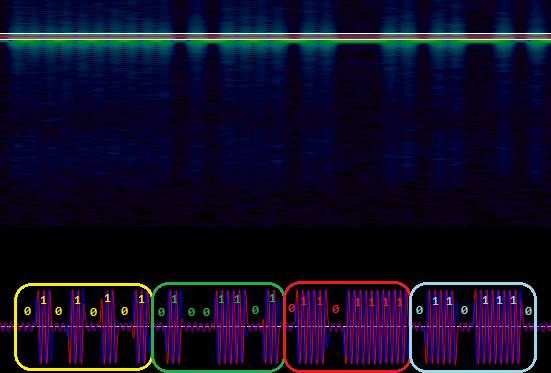
\includegraphics[width=0.85\textwidth ]{images_files/Aufgabe1_geschnitten.png}
	\caption{Bits und Bytes}
	\label{fig:YourLabe3}
\end{figure}

\begin{figure}[ht!]
\centering
	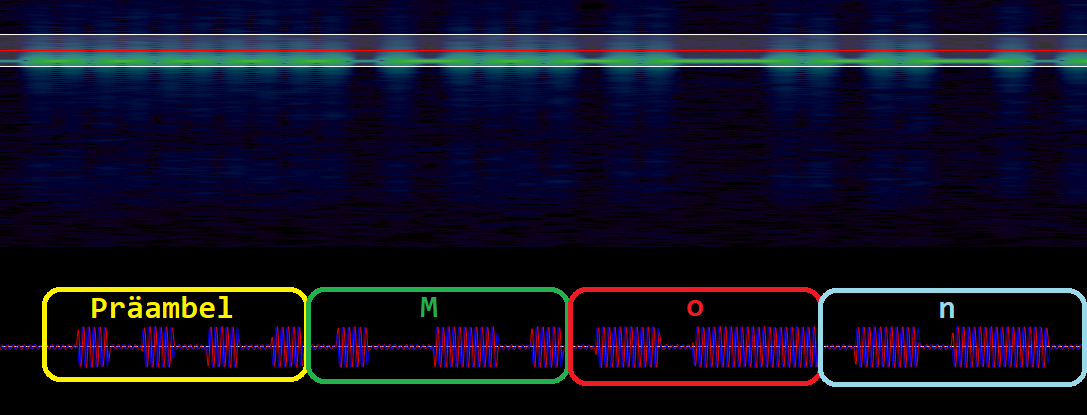
\includegraphics[width=0.85\textwidth ]{images_files/Aufgabe1-Demoduliert.png}
	\caption{Bytes ASCII kodiert}
	%\label{fig:YourLabe5}
\end{figure}

\newpage
Man erkennt, dass sich die Nachricht wiederholt.
\begin{figure}[ht!]
\centering
	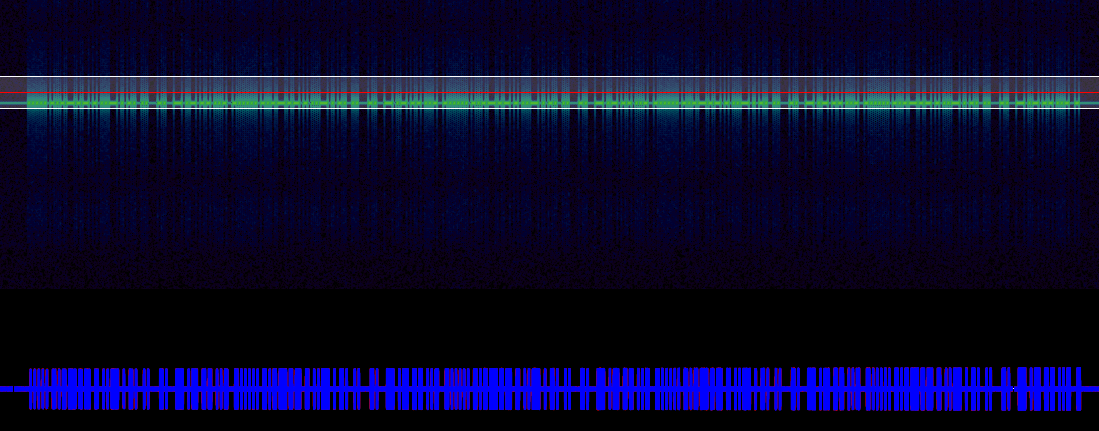
\includegraphics[width=1.04\textwidth ]{images_files/Aufgabe1-ganz.png}
	\caption{Gesamte Nachricht}
	%\label{fig:YourLabe5}
\end{figure}
\end{comment}



\section{Funkfernbedienungen}
\begin{comment}

Für diese Aufgabe wurde das Programm \textit{gqrx} mit folgenden Einstellungen verwendet:\\
	
\begin{figure}[ht]
\centering
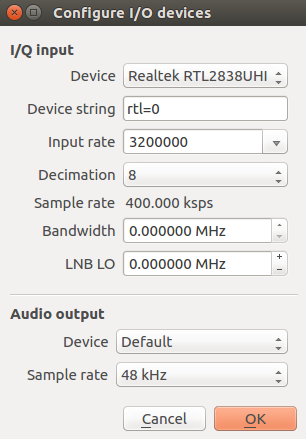
\includegraphics[scale=0.77]{images_files/A2_settings.png}
%\caption{Decimation}
\end{figure}
	
\begin{figure}[ht]
\centering
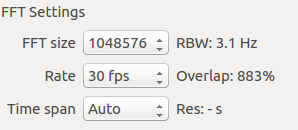
\includegraphics[scale=0.8]{images_files/A2_settings2.png}
\caption{FFT Size}
\end{figure}

\newpage
\subsection*{Signal 1}
	
\begin{itemize} 
	\item Modell: BMW 1er
	\item Mittenfrequenz: 868.877 MHz. Es gab jedoch weitere 			Frequenzberge.
	\item Screenshots:\\		
	\begin{minipage}{\linewidth}
	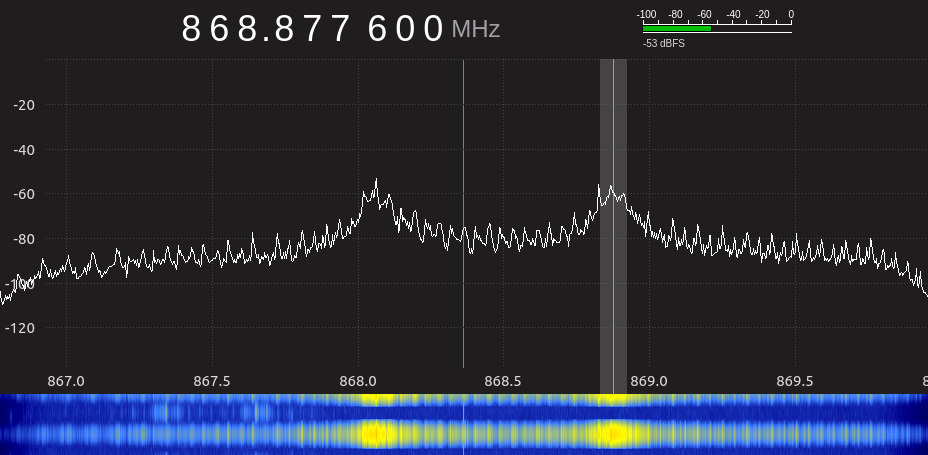
\includegraphics[width=1\textwidth]{images_files/A2_bmw_1_open_lock.png}
	\end{minipage}
	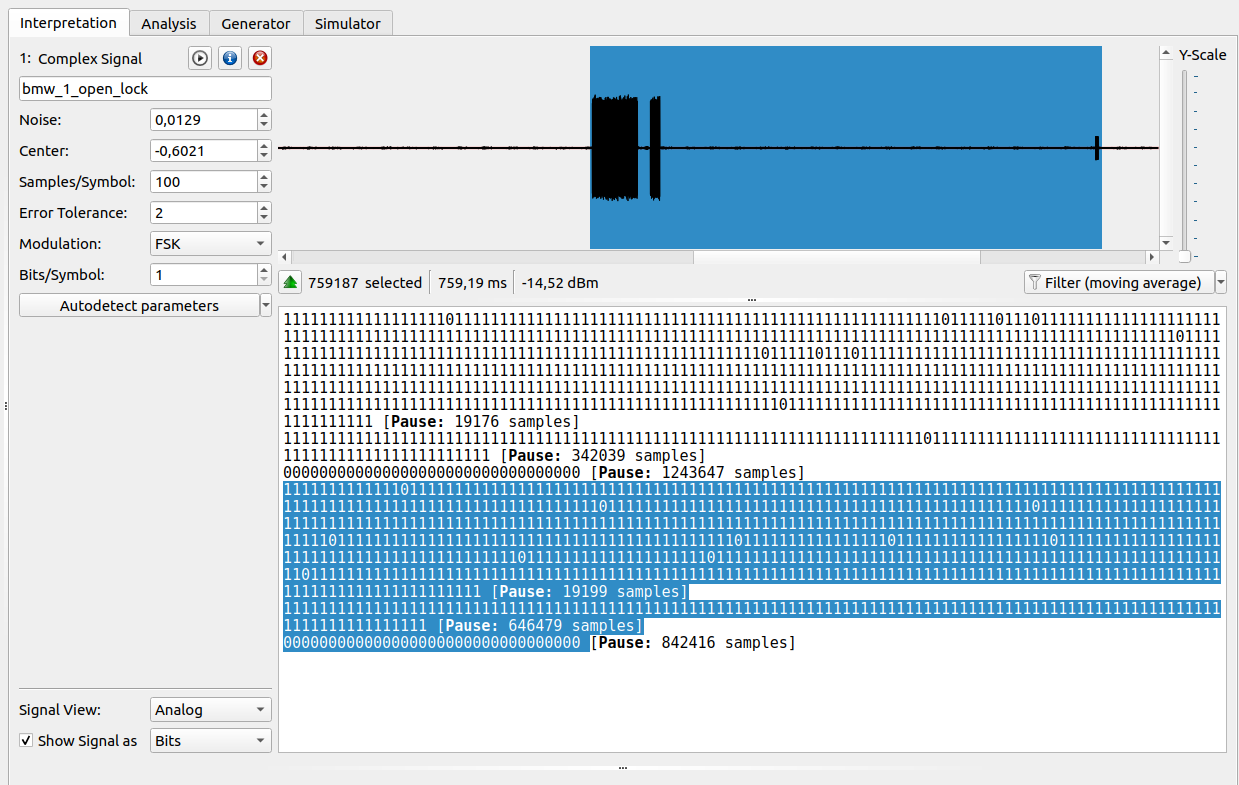
\includegraphics[width=1\textwidth]{images_files/Aufgabe2-Signal1-Zeitverlauf.png}
	
	\medskip
	Offenbar sendet die Fernbedienung auf mehreren Frequenzen\\
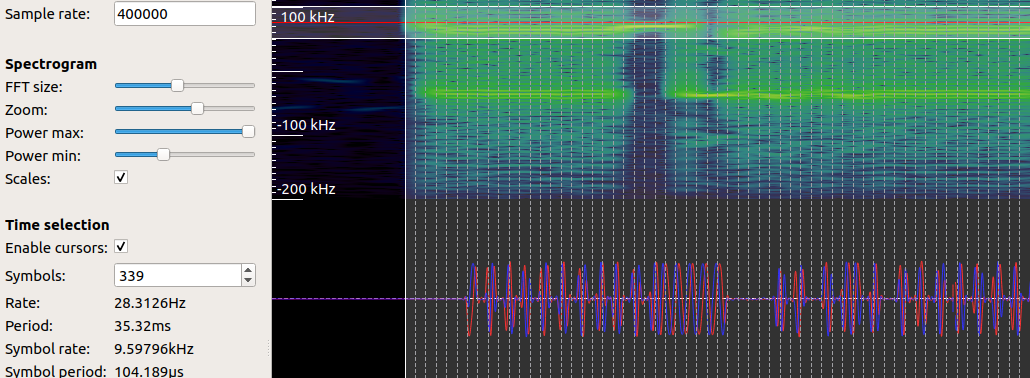
\includegraphics[width=1\textwidth]{images_files/A2_bmw_signal.png}
	\item Symbolrate:ca. 339 Symbole pro Signal - ca. 9.59kHz bei Sample rate von 400 000ksps
	\item Modulation: Laut URH autodetect FSK
\end{itemize}
\bigskip
	
\subsection*{Signal 2}

\begin{itemize}
	\item Modell: VW Caddy
	\item Mittenfrequenz: 434.397 MHz
	\item Screenshots:\\ \begin{minipage}{\linewidth}
	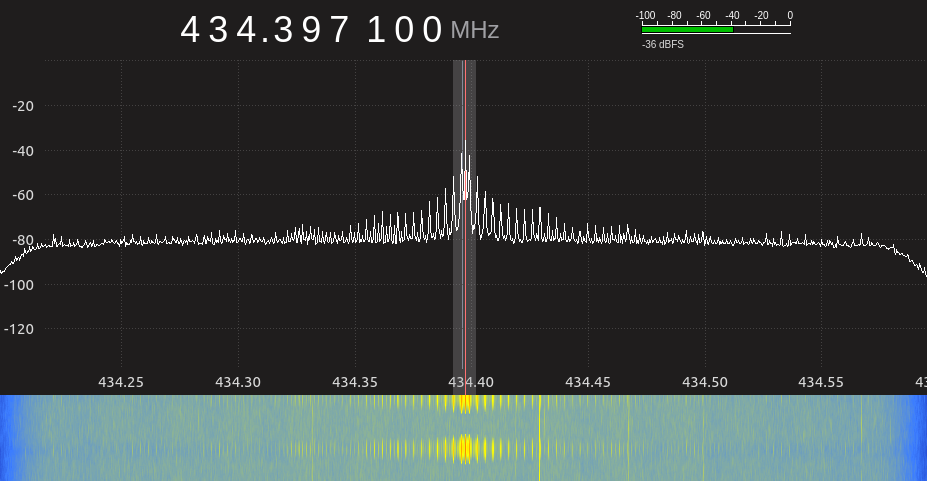
\includegraphics[width=1\textwidth]{images_files/A2_vw_caddy_open_lock.png}
	\end{minipage}
	\medskip
	Das Sendemuster hebt sich deutlich von dem des BMW ab
	\item Symbolrate:ca. 625 Symbole pro Signal - ca. 3.40kHz bei Sample rate
von 400 000ksps
	\item Modulation: ASK
	
		
	
	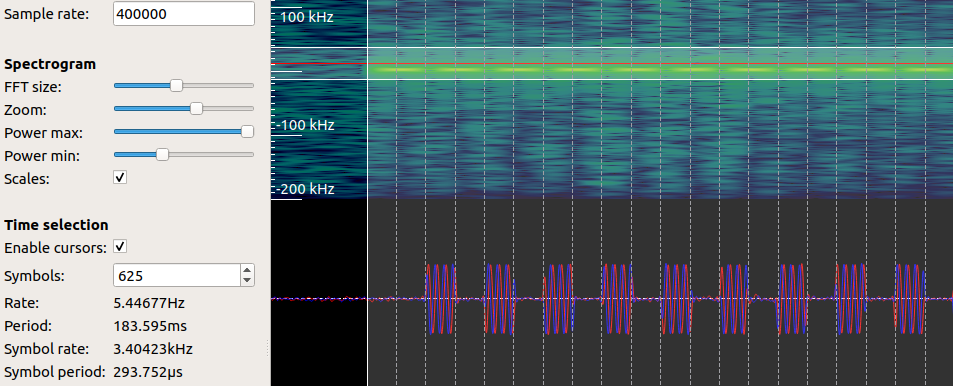
\includegraphics[width=1\textwidth]{images_files/A2_caddy_signal.png}
	
	
	
	\item Untersuchung: 
	\begin{itemize}
		\item ersten 430 Symbole \textit{1, 0} alternierend - 				Präambel
		\item letzten 204 Symbole fuer Oeffnung/Schliessung 				verantwortlich
		\item beide Signale unterscheiden sich nicht
	\end{itemize}
\end{itemize}	
\bigskip
	
\subsection*{Signal 3}	
	
\begin{itemize}
	\item Modell: Mercedes CLA
	\item Mittenfrequenz: 433.443 MHz
	\item Screenshots:\\ \begin{minipage}{\linewidth}
	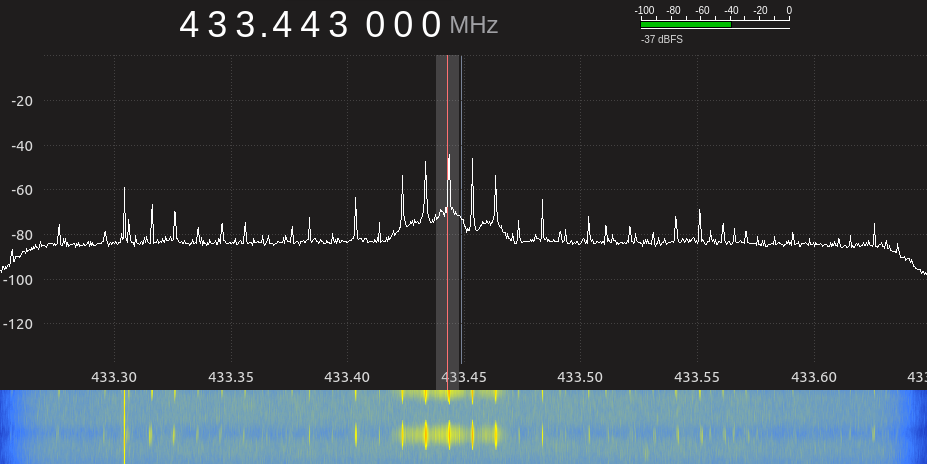
\includegraphics[width=1\textwidth]{images_files/A2_mercedes_cla_open_lock.png}
	\end{minipage}
	\item \begin{minipage}{\linewidth}
	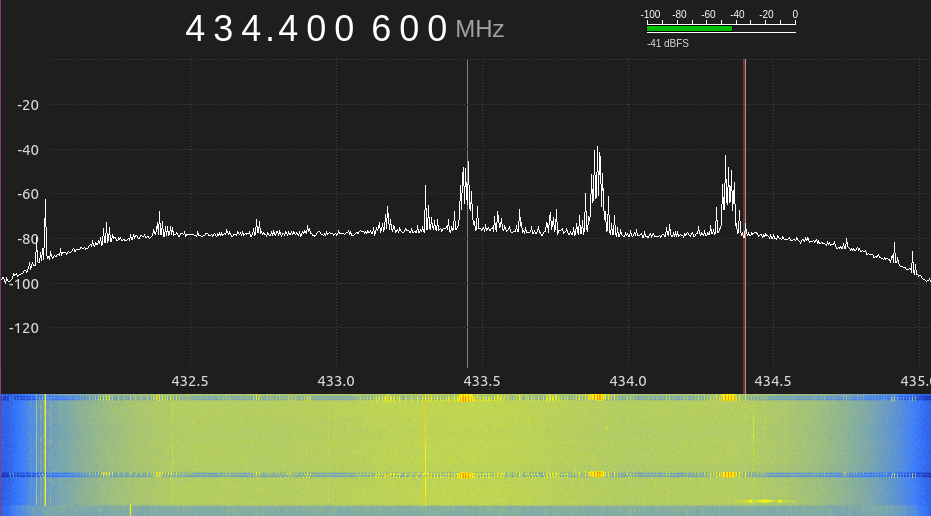
\includegraphics[width=1\textwidth]{images_files/A2_mercedes_zoom_out.png}
	\end{minipage}
	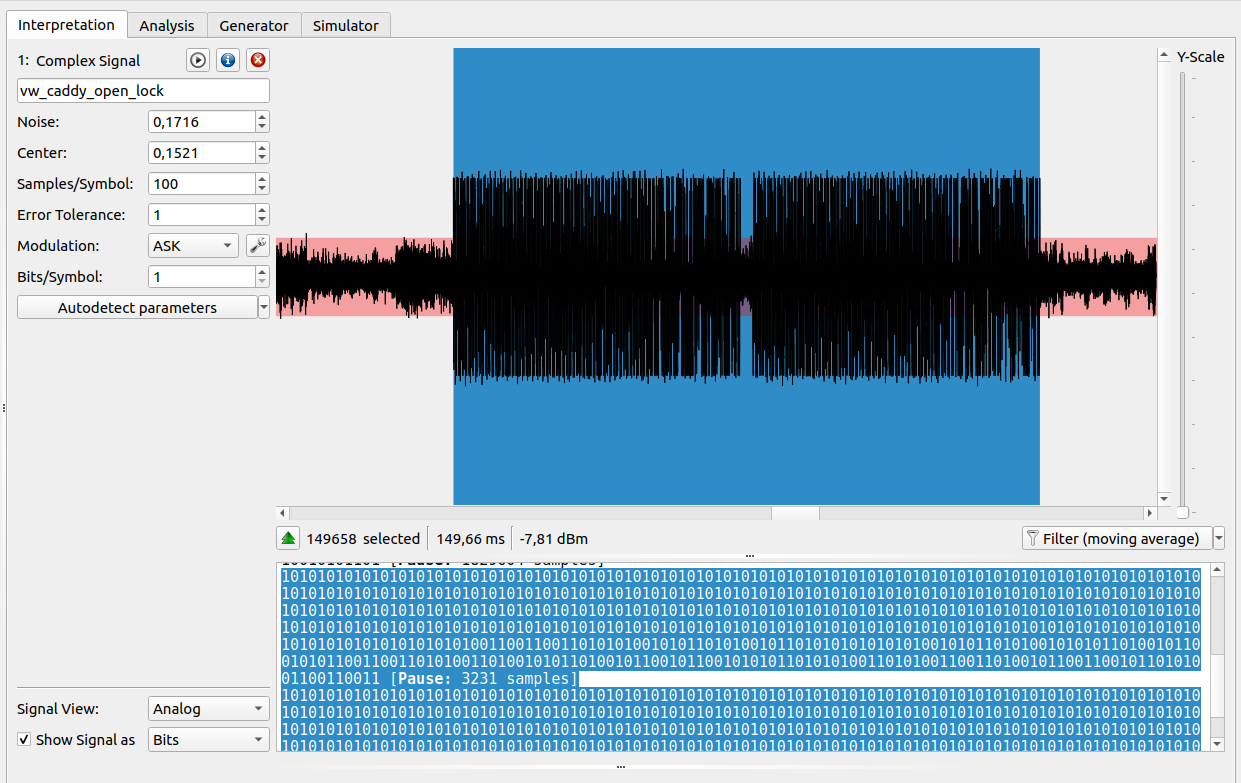
\includegraphics[width=0.98\textwidth]{images_files/Aufgabe2-Signal3-Zeitverlauf.png}
	\medskip
	Bei \textit{Decimation = 0} kann man erkennen, dass die Fernbedienung auf mehreren Frequenzen sendet
	\item Symbolrate: ca. 406 Symbole pro Signal - ca. 5.88kHz bei Sample
rate von 400 000ksps
	\item Modulation: Laut URH autodetect ASK
\end{itemize}
\bigskip

\newpage
\end{comment}


\section{Spectrum Sensing}
\begin{comment}

\begin{figure}[ht!]
\centering
	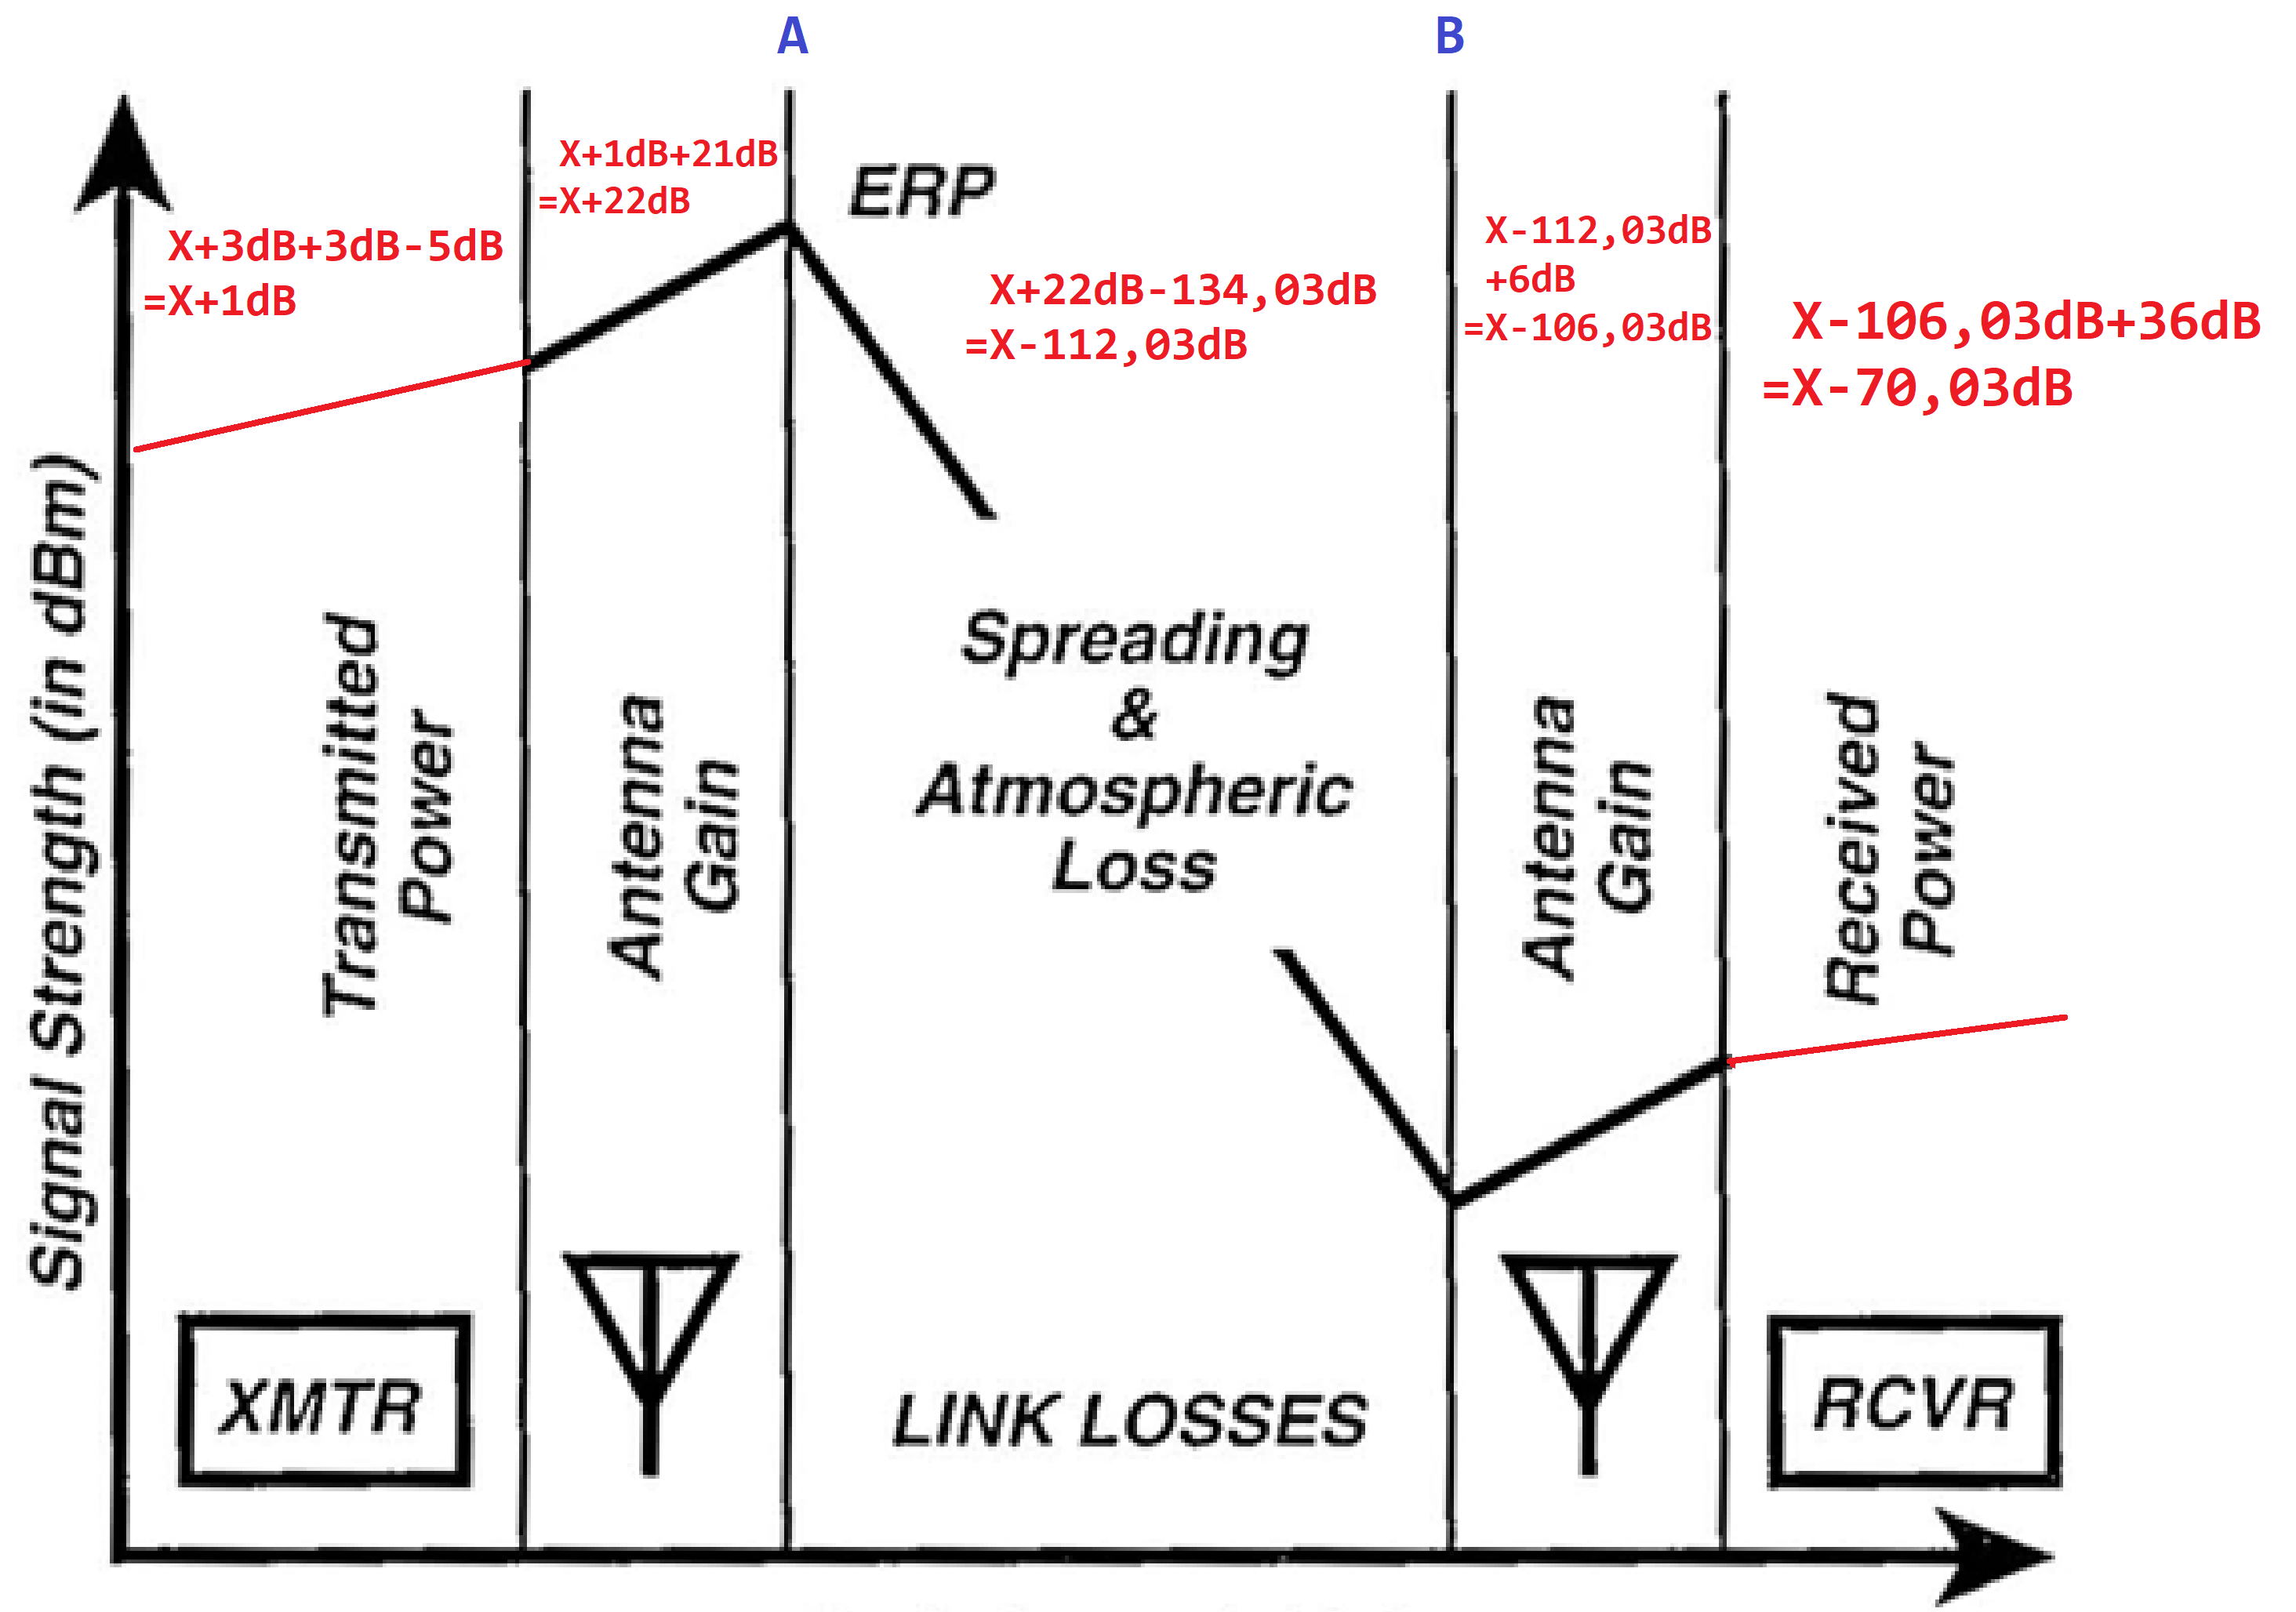
\includegraphics[width=1.05\textwidth ]{images_files/Aufgabe3_aktualisiert.png}
	\caption{Grafik 2}
	\label{fig:YourLabe4}
\href{https://www.amazon.de/EW-101-Electronic-Warfare-Library/dp/1580531695}{Quelle Skizze (Ohne farbige Notizen)}
\end{figure}



\subsection*{a)}
Maßeinheiten werden der besseren Übersicht halber ausgelassen in den Rechenwegen, aber nicht in den Endergebnissen selbst bei den Teilaufgaben a), b) sowie c)!\\\\
Orientiert man sich an der Formel aus dem mitgegebenen Dokument \textit{zsmfssg\_U1.pdf}, dann berechnet sich der Verlust in dB wie folgt:\\\\
$20*log_{10}(r*f*\dfrac{4\pi}{c})$, wobei r die Distanz in Metern, 120000, f die Frequenz in Hz, hier $10^{\hspace{0.8mm}9}$ und c
\\\\die Lichtgeschwindigkeit in m/s, also 299792458.\\\\
Wir setzen ein:\\
$20*log_{10}(120000*10^{\hspace{0.8mm}9}*\dfrac{4\pi}{299792458})\thickapprox134.03$. 
\subsubsection*{i) Matrikelnummer mit 22 am Ende}
Rechnung für die Matrikelnummer die mit 22 endet:\\\\
$X-134,03=22$
\\
$ \equiv 156,03 = X$.\\\\
Daraus folgt, dass X etwa 156,03 dBm stark sein sollte.
\subsubsection*{ii) Matrikelnummer mit 30 am Ende}
Rechnung für die Matrikelnummer die mit 22 endet:\\\\
$X-134,03=30$
\\
$ \equiv 164,03 = X$.\\\\
Daraus folgt, dass X etwa 164,03 dBm stark sein sollte.

\subsection*{b)}
\glqq Nehmen Sie an, dass das Signal mit 100 dBm gesendet wird. Der Empfänger soll nach allen Verlusten/Verstärkungen ein 60 dB Signal erhalten. Wie muss die Frequenz geändert werden, damit dieses Ziel erreicht wird?\grqq\\\\


Wie in Abilldung~\ref{fig:YourLabe4} auf  Seite \hspace{1mm}\pageref{fig:YourLabe4} deutlich wird "gewinnt" \hspace{1mm} das Signal von Punkt B bis hin zur fertigen Verarbeitungen 42\hspace{0.6mm} dBm. Das heißt, nachdem das Signal bei B ankommt, kommen noch 6\hspace{0.6mm} dBi
Gewinn durch die Antenne hinzu und 42\hspace{0.6mm} dB durch den Verstärker. Sei 100\hspace{0.6mm}dBm die Stärke des ausgestrahlten Signals bei Punkt A. Gesucht ist f.\\\\
Es soll gelten:\\\\
$100\hspace{1mm}-20*log_{10}(120000*f*\dfrac{4\pi}{299 792 458}) + 6 +36 = 60\hspace{1mm}$
\\~\\\\
$\equiv 
-20*log_{10}(120000*f*\dfrac{4\pi}{299 792 458})=-82$
\\~\\\\
$\equiv 
log_{10}(120000*f*\dfrac{4\pi}{299 792 458})=4,1$
\\~\\\\
$\equiv
\dfrac{ln(\dfrac{480 000\pi*f}{299 792 458})}{ln(10)}=4,1  $
\\~\\\\
$\equiv
ln(\dfrac{480 000\pi*f}{299 792 458})=4,1*ln(10)$
\\~\\\\
$\equiv 
ln(\dfrac{480 000\pi*f}{299 792 458}) =4,1*ln(10)=ln(10^{\hspace{0.6mm}4,1})$
\\~\\\\
$\equiv
\dfrac{480000\pi*f}{299 792 458}=10^{\hspace{0.6mm}4,1}$
\\~\\\\
$\equiv 
f=\dfrac{10^{\hspace{0.6mm}4,1}*299792458}{480000\pi}$
\\~\\\\
$\equiv 
f=\dfrac{10^{\hspace{0.6mm}4,1}*149896229}{240000\pi}\thickapprox
2502819,86 $
\\~\\\\

Check:\\\\
$100\hspace{0.6mm}dBM-20*log_{10}(120 000*\dfrac{10^{\hspace{0.6mm}4,1}*149896229}{240000\pi}*\dfrac{4\pi}{299 792 458})\hspace{0.6mm}dBM +6\hspace{0.6mm}dBM +36\hspace{0.6mm}dBM =60\hspace{0.6mm}dBM$
\\~\\\\
Check erfolgreich. Das heißt, es muss mit der Frequenz von etwa 2502819,86 Hz, beziehungsweise 2,5 MHz gesendet werden. 




\subsection*{c)}

\glqq Das Signal wird nun wieder mit einer Frequenz von 1 GHz gesendet. Wie muss sich die Entfernung
von Sender/Empfänger ändern, sodass der Empfänger nach allen Verlusten/Verstärkungen ein Signal
mit Leistungspegel 60 dB erhält? Nehmen Sie dafür erneut an, dass das Signal mit 100 dB gesendet
wurde.\grqq \\\\

Gesucht ist r. Es soll gelten:\\~\\
$100-20*log_{10}(r*10^{\hspace{0.7mm}9}*
\dfrac{4\pi}{299 792 458})+6+36=60$
\\~\\\\
$\equiv
log_{10}(r*10^{\hspace{0.7mm}9}*
\dfrac{4\pi}{299792458})=4,1$
\\~\\\\
$\equiv
\dfrac{ln(\dfrac{2*10^{\hspace{0.6mm}9}\pi*r}{149 896 229})}{ln(10)}=4,1$ \\~\\\\
$\equiv
ln(\dfrac{2*10^{\hspace{0.6mm}9}\pi*r}{149 896 229})=4,1*ln(10)$
\\~\\\\
$\equiv
ln(\dfrac{2*10^{\hspace{0.6mm}9}\pi *r}{149 896 229})=ln(10^{\hspace{0.6mm}4,1})$
\\~\\\\
$\equiv
\dfrac{2*10^{\hspace{0.6mm}9}\pi*r}{149 896 229}=10^{\hspace{0.6mm}4,1}$
\\~\\\\
$\equiv
r = 10^{\hspace{0.6mm}4,1}*\dfrac{149 896 229}{2*10^{\hspace{0.6mm}9}\pi}$
\\~\\\\
$=\dfrac{149896229}{2*10^{\hspace{0.6mm}4,9}\pi}
\thickapprox 300,34$
\\~\\\\

Check:\\\\
$100\hspace{0.6mm}dBM-20*log_{10}(\dfrac{149896229}{2*10^{\hspace{0.6mm}4,9}\pi}*10^{\hspace{0.6mm}9}*\dfrac{4\pi}{299 792 458})\hspace{0.6mm}dBM +6\hspace{0.6mm}dBM +36\hspace{0.6mm}dBM =60\hspace{0.6mm}dBM$
\\~\\\\
Check erfolgreich. Das heißt, die Distanz muss etwa 300,34 m betragen.

\subsection*{d)}

\glqq In der Vorlesung haben Sie zwei Approximierungen gelernt, wie man Dezibel Werte ohne Logarithmus berechnen kann.\\\\
\begin{center}
$3\hspace{0.8mm}dB \longmapsto 2 : 1$\\
$10\hspace{0.8mm}dB \longmapsto 10 : 1$\\
\end{center}
Berechnen Sie die approximierten Absolutbeträge von 113 dB jeweils mit einer der beiden Approximationen und vergleichen Sie diese mit dem korrekten Wert. Sind die Approximationen gut? Begründen Sie Ihre Antwort. Können Sie mit einer Kombination aus beiden Approximationen einen besseren
Wert erreichen?\grqq \\\\

Bekannt ist aus $ \textit{zsmfssg\_{}U1.pdf:}$\\
$ 10*log_{10}(Faktor) = dB $\\\\
Benutzt man \href{http://www.sengpielaudio.com/Rechner-FaktorVerhaeltnisPegelDezibel.htm}{http://www.sengpielaudio.com/Rechner-FaktorVerhaeltnisPegelDezibel.htm} ergibt sich der richtige Faktor mit 199526231496.8883 was sich übrigens mit $10^{11.3}$ berechnen lässt.



\subsubsection*{Methode 1}
$113=37*3+2 \rightarrow 2^{37}$\\
Der Rest ist somit 2.\\

Kontrolle:\\
$10*log_{10}(2^{37})= 111.38\hspace{0.8mm}dB$\\
Je kleiner der Differenzbetrag mit dem richtigen Faktor, desto besser:\\
$10^{11.3}-2^{37} \thickapprox 62087278025$



\subsubsection*{Methode 2}

$113=11*10+3 \rightarrow 10^{11} $\\
Der Rest ist somit 3.\\

Kontrolle:\\
$10*log_{10}(10^{11})= 110\hspace{0.8mm}dB$\\
Je kleiner der Differenzbetrag mit dem richtigen Faktor, desto besser:\\
$10^{11.3}-10^{11} \thickapprox 99526231497$
								



\subsubsection*{Kombination aus beiden Approximationen }
$113=11*10+1*3 \rightarrow {10^{11}}*2^1=2*10^{11}$\\
Der Rest ist somit 0.\\


Kontrolle:\\
$10*log_{10}(2*10^{11})\thickapprox 113.01\hspace{0.8mm}dB$\\
Je kleiner der Differenzbetrag mit dem richtigen Faktor, desto besser:\\
$\vert \hspace{0.8mm} 10^{11.3}-2*10^{11}\hspace{0.8mm}\vert \thickapprox 473768503$\\\\

Wie in Abilldung~\ref{fig:YourLabe7} auf  Seite \hspace{1mm}\pageref{fig:YourLabe7}	klar wird, ist hier die Kombination am besten, gefolgt von Methodik 1. Methodik 2 ist in diesem Fall am schlechtesten. Wenn man als Kriterium nimmt, dass Methodiken 1 und 2 auf den richtigen ganzen dB Wert kommen, dann sind es keine guten Approximationen. Wenn relativ genaue Werte benötigt werden, eignen sich diese nicht, aber sie können hilfreich sein um grob abzuschätzen. Wie gesagt ist die Kombination am besten,
wo auch der Rest mit 0 am kleinsten war. Methodik 1 hatte den zweit kleinsten Rest mit 2, gefolgt von Methodik 2 mit Rest 3, was mathematisch gesehen kein Zufall war.
					  


%dB <-c(111.38, 110, 113.01)
%Differenzbeträge <-c(62087278025, 99526231497, 473768503)

%d <-cbind(dB,Differenzbeträge)
%rownames(d)<-c("Methodik 1", "Methodik 2", "Kombination")
%d

\begin{figure}[ht!]
\centering
	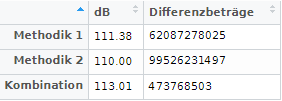
\includegraphics[width=1.\textwidth ]{images_files/Aufgabe-3d).png}
	\caption{Vergleich}
	\label{fig:YourLabe7}
\end{figure}

\newpage
%Beispielbilder:
%\begin{figure}[ht!]
%	\centering
%	\includegraphics[width=0.9\textwidth ]{YourImage}
%	\caption{Your Caption}
%	\label{fig:YourLabel}
%\end{figure} 

%Or you can use wrapfigure
%\begin{wrapfigure}{l}{0.25\textwidth}
%	\includegraphics[width=0.2\textwidth ]{Image}
%	\caption{cap}
%	\label{fig:lab}
%\end{wrapfigure}


\end{comment}

\section{Reading assignment}

\subsection{a)} 
Siehe Seite 36 des Papers sollen damit \textit{resource 
depletion attacks} und \textit{masquerade attacks} 
abgewehrt werden.


\subsection{b)} 
Siehe Seite 37 des Papers haben Signalprints die folgenden 
Eigenschaften:

\begin{itemize}
	\item Sie sind schwer zu \textit{spoofen} 
	\item Sie weisen eine starke Korrelation in Hinblick auf ihre 
	physikalische Umgebung auf
	\item Über mittlere Zeitdauern variieren sie nur leicht 
\end{itemize}


\subsection{c)} 

\subsubsection*{Node Induction}
Da der Sender nur mithilfe des empfangenen Signalprints,
welches mit dem Referenz-Signalprints verglichen wird, 
identifiziert werden kann, muss das voraussetzen, dass 
das Referenz-Signalprint existiert. Falls jedoch eine 
Node zum ersten mal mit dem Netzwerk interagiert, fehlt 
logischerweise dieses Referenz-Signalprint, was das 
Identifizieren dieser Node nicht möglich macht. 
Wenn eine Node sich dem Netzwerk anschließen will, legt 
sie offen auf welchen Kanälen sie die restlichen 
Übertragungen senden wird. Die Empfänger stellen sich 
darauf ein und messen ihre jeweiligen RSSI Werte, die 
daraufhin über das Netzwerk verteilt werden. 

\subsubsection*{Frequent Hello Messages}
Aufgrund der kontinuierlichen Batterieentladung sinkt 
die Übertragunsstärke zunehmend, was zur Folge hat, 
dass die RSSI-Werte mit der Zeit abnehmen. 
Als Konsequenz wird der Vergleich der RSSI-Werte mit 
dem Signalprint nach einer gewissen Zeit beeinträchtigt 
und somit die Identifikation.
Im Allgemeinen kann die Entladungsrate nicht ohne Weiteres 
vom Empfänger vorrausgesagt werden, da es von der Ladung 
des Senders abhängt. Deshalb wird das regelmäßige Versenden 
von  \glqq hello\grqq \hspace{0.5mm} Packeten empfohlen.
Immer wenn ein Empfänger eine Übertragung eines Senders erhält, 
vergleicht dieser dann den empfangenen RSSI-Wert mit dem des 
Referenz-Signalprints. Erreicht die Differenz eine gewisse 
Größe, wird die Generierung eines neuen Referenz-Signalprints 
angefordert. Oft reicht der Verkehr von genuinen Übertragungen 
aus, aber ist das nicht der Fall müssen \glqq hello\grqq
\hspace{0.5mm}Packete übertragen werden zur erfolgreichen 
Verifizierung der RSSI-Werte.


\subsubsection*{Data Transmission}
Nicht jede Datenübertragung wird mithilfe eines Signalprints 
verifiziert. Je mehr Empfänger zusammenarbeiten um ein 
Signalprint zu generieren, desto höher die Verlässlichkeit 
des Signalprints. Es kann passieren, dass zu einem Zeitpunkt 
nicht genug Empfänger auf einen bestimmten Kanal eingestimmt 
sind um einen ausreichend verlässlichen Signalprint zu erhalten. 
Deshalb wird eine Methodik bestehend aus zwei Schritten verwendet:
\begin{itemize}
	\item Das Netzwerk hält Ausschau nach verdächtiger Aktivität
	\item Falls so eine Aktivität bemerkt wurde, stimmt das Netzwe 
	eine ausreichende Anzahl an Empfängern auf die entsprechenden 
	Kanäle ein und ein Signalprint wird erzeugt
\end{itemize}



%Als Beispiel für einen Hyperlink übrig gelassen
\begin{comment}
\href{https://www.pc-magazin.de/ratgeber/das-muessen-sie-ueber-lte-wissen-1277030.html}{(hier klicken)}
\end{comment}
\end{document}